\section{Results}
\label{section:slr_result}

We carried out a systematic literature review (SLR).
We summarise the results of our SLR as ``undetermined''.
We make this statement because the review design was not wholly appropriate for the problem domain.

We could not find a quality assessment checklist that adequately dealt with design science research (DSR) studies.
This inadequacy proved problematic, as most of the primary studies were DSR studies.
Therefore, what follows should be considered the results of a quasi-SLR, with the quality assessment stage ignored.

\subsection{Papers Selected}
We logged the details of what we describe in this section in appendix \ref{Appendix:SLRLog}.

Figure \ref{fig:search_results}, on the following page, shows the results of the five iterations that the search went through.
Out of 173 results, we had 50 papers that provisionally seemed to pass our inclusion and exclusion criteria from our initial search.
From the initial 50, we added 18 papers from a possible 109 in our first iteration of forward and backwards snowballing.
The next snowballing iteration returned three papers that matched our criteria.
The third round of snowballing had no papers matching our criteria and thus terminated this stage of selection.

\begin{figure}
    \centering
    \fbox{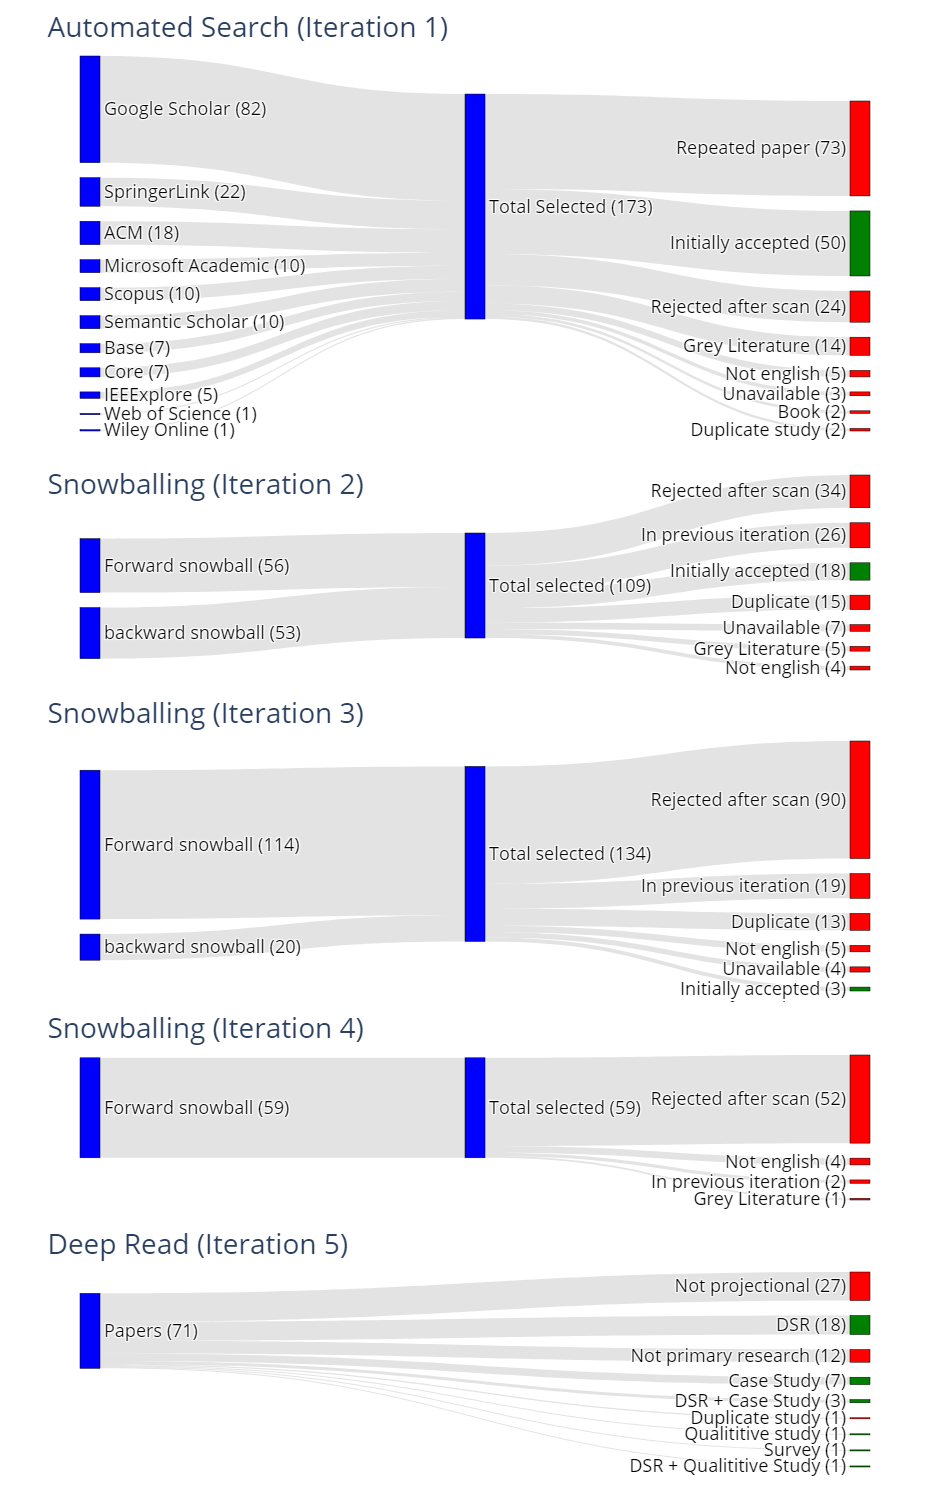
\includegraphics[width=0.95\textwidth]{Sections/images/search_sankey-2.png}}
    \caption{Search results}
    \label{fig:search_results}
\end{figure}

Our final selection iteration involved a deeper scan of the remaining 71 papers.
In this stage, we rejected 12 papers that were not primary research and one paper which reported on an already represented study.
Further, we rejected twenty-seven papers that were, on closer reading, not about projectional editing.

This final selection filter left us with 31 papers before the quality assessment filter. 

\subsubsection{Sensitivity and Precision}
As a curio, we reappropriated Zhang's\cite{Zhang_2011} ideas of sensitivity and precision and applied them to the search engines rather than search strings.
We calculate the values for sensitivity and precision of the search engines as follows:
\[
        sensitivity = \frac{\#\;retrieved\;relevant\;studies}{\#\;all\;relevant\;studies} \;100\%
\]

\[
        precision = \frac{\#\;retrieved\;relevant\;studies}{\#\;studies\;retrieved} \;100\%
\]

Table \ref{table:sensitivity_precision} show that Google Scholar had the highest sensitivity, returning 22 of the 31 chosen studies.
This sensitivity came at the cost of a considerable proportion of false positives.
Microsoft Academic and SpringerLink were the joint-most precise, with half of their search results ending up in the final roster.
With the second-highest count of documents, the second-highest sensitivity, and joint highest precision, SpringerLink would appear to be the best all-around search engine for this field.
However, these figures are skewed by several of their articles coming from a single collection specifically about projectional editing.

\begin{table}[h]
    \begin{center}
        \begin{tabular}{ | l | c | c | c | c |} 
            \hline
            Search engine/library     & original \# & selected \# & sensitivity & precision\\
            \hline
            \hline
            ACM                        & 18          & 3           & 10\%        &  16\%    \\
            BASE                       & 7           & 3           & 10\%        &  43\%    \\
            CORE                       & 7           & 1           &  3\%        &  14\%    \\
            Google Scholar             & 82          & 22          & 71\%        &  27\%    \\
            IEEExplores                & 5           & 2           &  6\%        &  40\%    \\
            Microsoft Academic         & 10          & 5           & 16\%        &  50\%    \\
            Science.gov                & 0           & 0           &  0\%        &   0\%    \\
            SCOPUS                     & 10          & 3           & 10\%        &  30\%    \\
            Semantic Scholar           & 10          & 4           & 13\%        &  40\%    \\
            SpringerLink               & 22          & 11          & 35\%        &  50\%    \\
            Wiley Online               & 1           & 0           &  0\%        &   0\%    \\
            Web of Science             & 1           & 0           &  0\%        &   0\%    \\
            \hline
        \end{tabular}
    \end{center}
    \caption{Search engine sensitivity and precision}
    \label{table:sensitivity_precision}
\end{table}

\subsection{Quality Assessment}
During this quality assessment, we discovered that two of the papers we had initially categorised as primary studies were, in fact, proposals, and thus we removed them from our analysis.
Using the quality assessment checklists developed by Crombie et al.\cite{crombie1997pocket}, shown in appendix \ref{appendix:QualityAssesmentChecklist}, we examined the remaining 29 papers, which on the surface represented 35 primary studies.

Unfortunately, there were no checklists for DSR studies.
We, unsuccessfully, searched for an appropriate quality assessment checklist for DSR studies.
We did not find a suitable checklist and did not consider ourselves suitably qualified to make one.
So, we used the quality assessment checklist for case studies to assess the DSR studies.

We used a rudimentary scoring system of +1 value for positive answers, 0 for undetermined, and -1 for negative answers.
We arbitrarily defined that any study with an overall score greater than 0 was high enough quality to be part of our final analysis.

Unfortunately, we only found 6 out of 37 studies of high enough quality to pass this filter with this scoring.
Thus, we had to choose between changing our scoring, only using these six studies, terminating the SLR or ignoring the QA findings.

Changing a method until it gave the desired answer seemed unscientific to us.
Six studies seemed too few to give an overview of a field.
Abandoning the SLA seemed the correct course of action.
However, as we still wanted an overview, we decided to take a different course.
We accept that what follows is no longer an SLA. 
We titled it a Quasi-SLA, which is like an SLA, which ignores the quality assessment results.

We could not reconcile that 84\% of studies were high-quality enough to appear in recognised scientific journals yet were not of high enough quality to pass our SLR QA stage.
After considering this disconnect, we found two significant threats to the validity of the Quality Assessment stage.
The first is that a single researcher with no previous experience executed the QA stage.
The second is that either case study checklists are inappropriate for DSR studies or that DSR studies are inappropriate for SLRs.

\subsection{Analysis}
\label{section:slr_analysis}

After Identifying the primary studies, we extracted data.
Appendix \ref{appendix:DataExtraction} shows the forms containing the raw extracted data.
Figure \ref{fig:study_types} shows that most of the primary studies in our review were DSR studies.

\begin{figure}[h]
    \centering
    \fbox{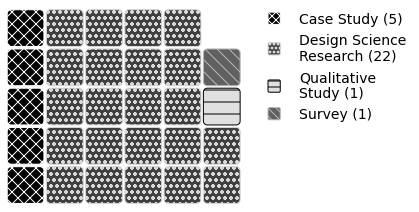
\includegraphics[width=0.45\textwidth]{Sections/images/pie_study_type4.png}}
    \caption{Study types}
    \label{fig:study_types}
\end{figure}

\subsubsection{Tools Used}

We split the studies to see which were to do with purely research projects and which were researching using already publicly available commercial or open-source products.
To calculate this, we removed one primary study, a survey, as it covered many tools and options, but none of which was in-depth.
Figure \ref{fig:public_vs_research} shows that over 80\% of the projects were studying already existing publicly available options.

Of the publicly available software studies, we wanted to know which software attracted the most academic interest.
Figure \ref{fig:public_programs} shows that 74\% of the studies into projectional editing that used a publicly available product used JetBrains MPS.

\begin{figure}[h]
    \centering
    \fbox{\begin{minipage}{0.5\textwidth}
            \centering
            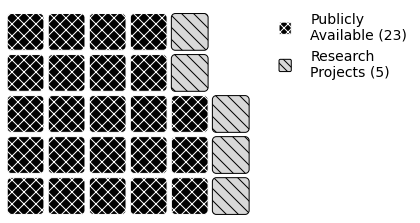
\includegraphics[width=0.85\textwidth]{Sections/images/pie_projectional_publicvsresearch3.png}
            \caption{Public vs research}
            \label{fig:public_vs_research}
        \end{minipage}\hfill
        \begin{minipage}{0.5\textwidth}
            \centering
            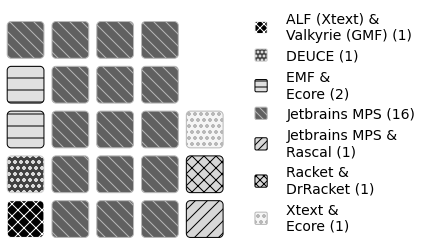
\includegraphics[width=0.85\textwidth]{Sections/images/pie_projectional_publicprograms3.png} 
            \caption{Publicly available programs}
            \label{fig:public_programs}
        \end{minipage}
    }
\end{figure}

\subsubsection{Sentiment}

In this study, we included all 29 papers.
We tagged each section from those papers that talked about projectional editing.
We then broke each section into sentences and ran those sentences through a sentiment analyser as described in section \ref{section:dataExtraction}.
We show the outcome of this sentiment analysis in figure \ref{fig:sentiment_analysis} on page \pageref{fig:sentiment_analysis}. 
The charts show the relationship between the positive, neutral, and negative sentiment outcomes.
On the y-axis, we have an Id for the papers examined. 
We show the keys linking the Ids to the paper names in table \ref{table:paper_key}, on page \pageref{table:paper_key}, the page following the charts.

\begin{figure}
    \centering
    \fbox{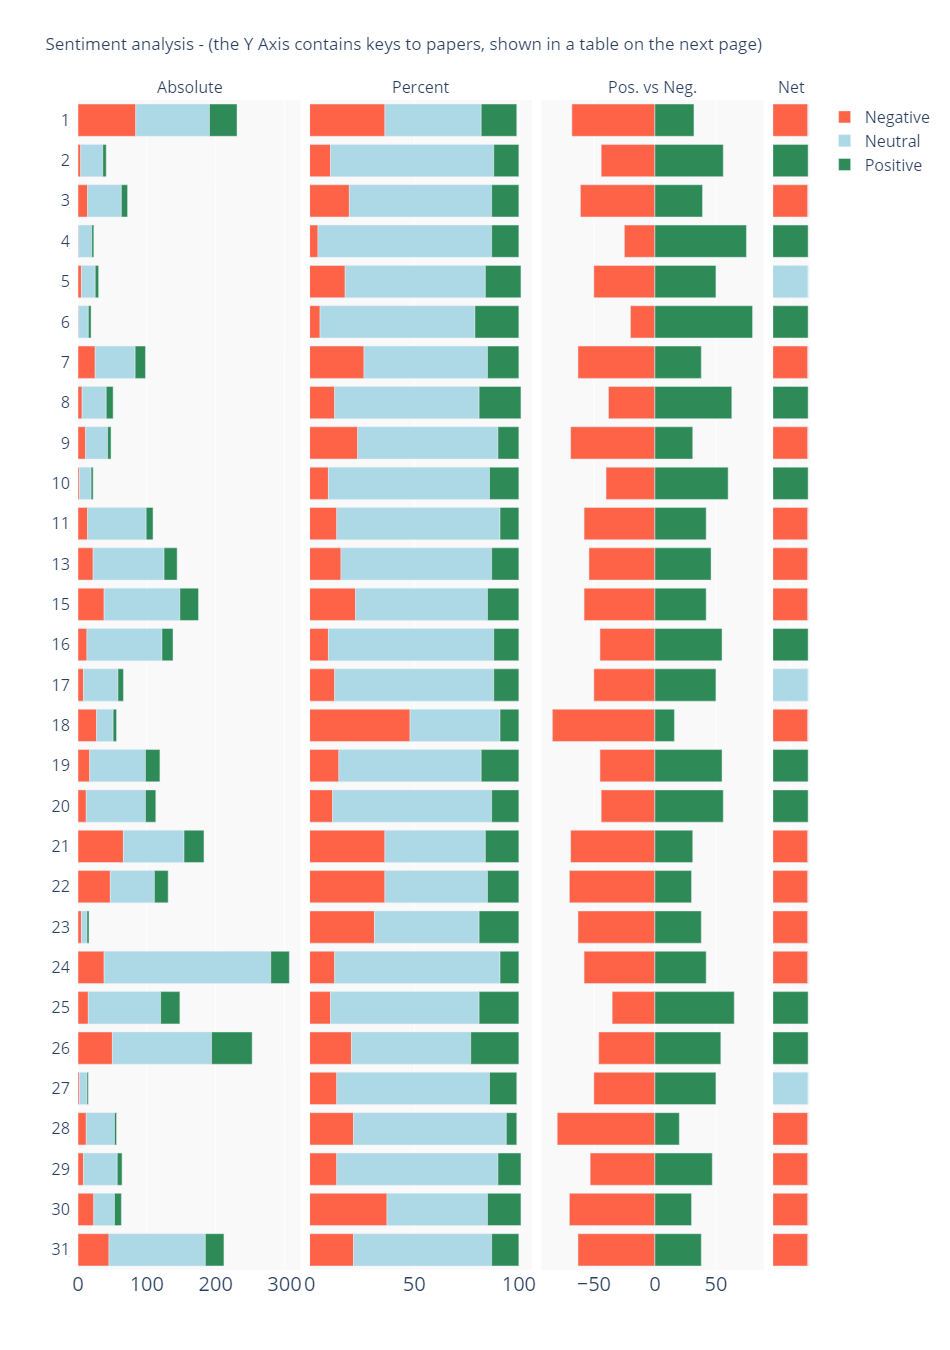
\includegraphics[width=0.95\textwidth]{Sections/images/sentiment_analysis4.png}}
    \caption{Sentiment analysis}
    \label{fig:sentiment_analysis} 
\end{figure}
 
\begin{table}
    \begin{center}
        \begin{tabular}{ |c  c|l | } 
            \hline
            Id  &                                        & Paper name                                                                  \\
            \hline
            1   &  \cite{voelterdomain_SLR}              & A domain-specific language for payroll calculations: A case study at DATEV  \\ \hline
            2   &  \cite{schropfer2021framework_SLR}     & A framework for projectional multi-variant model editors                    \\ \hline
            3   &  \cite{schropfer2020generic_SLR}       & A generic projectional editor for EMF models                                \\ \hline
            4   &  \cite{bucchiarone2019model_SLR}       & A model-driven approach towards automatic migration to microservices        \\ \hline
            5   &  \cite{meacham2020adaptivevle_SLR}     & AdaptiveVLE: An integrated framework for personalized online education      \\
                &                                        & using MPS JetBrains domain-specific modeling environment                    \\ \hline
            6   &  \cite{andersen2020adding_SLR}         & Adding interactive visual syntax to textual code                            \\ \hline
            7   &  \cite{addazi2021blended_SLR}          & Blended graphical and textual modelling for UML profiles: A                 \\
                &                                        & proof-of-concept implementation and experiment                              \\ \hline
            8   & \cite{meacham2020classification_SLR}   & Classification algorithms framework (CAF) to enable intelligent systems     \\
                &                                        & using JetBrains MPS domain-specific languages environment                   \\ \hline
            9   & \cite{furtado2021dsl_SLR}              & DSL based approach for building model-driven questionnaires                 \\ \hline
            10  & \cite{beckmann2020efficient_SLR}       & Efficient editing in a tree-oriented projectional editor                    \\ \hline
            11  & \cite{kolovos2020efficient_SLR}        & Efficient generation of graphical modelviews via lazy model-to-text         \\
                &                                        & transformation                                                              \\ \hline
            13  & \cite{bucchiarone2021engineering_SLR}  & Engineering gameful applications with MPS                                   \\ \hline
            15  & \cite{ratiu2021fasten_SLR}             & Fasten: An extensible platform to experiment with rigorous modeling of      \\
                &                                        & safety-critical systems                                                     \\ \hline
            16  & \cite{lafontant2020gentleman_SLR}      & Gentleman: A light-weight web-based projectional editor generator           \\ \hline
            17  & \cite{schropfer2019integrating_SLR}    & Integrating UML and ALF: An approach to overcome the code generation        \\
                &                                        & dilemma in model-driven software engineering                                \\ \hline
            18  & \cite{santos2020javardise_SLR}         & Javardise: A structured code editor for programming pedagogy in Java        \\ \hline
            19  & \cite{schindler2021jetbrains_SLR}      & JetBrains MPS as core DSL technology for developing professional digital    \\
                &                                        & printers                                                                    \\ \hline
            20  & \cite{simi2021learning_SLR}            & Learning data analysis with metaR                                           \\ \hline
            21  & \cite{stotz2021migrating_SLR}          & Migrating insurance calculation rule descriptions from Word to MPS          \\ \hline
            22  & \cite{munk2020model_SLR}               & Model-based safety assessment with SYSML and component fault trees:         \\
                &                                        & Application and lessons learned                                             \\ \hline
            23  & \cite{bucchiarone2020papyrus_SLR}      & Papyrus for gamers, let’s play modeling                                     \\ \hline
            24  & \cite{merino2021projecting_SLR}        & Projecting textual languages                                                \\ \hline
            25  & \cite{cuinat2020specedit_SLR}          & SpecEdit: Projectional editing for TLA+ specifications                      \\ \hline
            26  & \cite{prinz2021teaching_SLR}           & Teaching language engineering using MPS                                     \\ \hline
            27  & \cite{barash2021teaching_SLR}          & Teaching MPS: Experiences from industry and academia                        \\ \hline
            28  & \cite{hempel2020tiny_SLR}              & Tiny structure editors for low, low prices! (generating GUIs from           \\
                &                                        & toString functions)                                                         \\ \hline
            29  & \cite{negm2020towards_SLR}             & Towards ontology-based domain specific language for internet of things      \\ \hline
            30  & \cite{lubin2020type_SLR}               & Type-directed program transformations for the working functional            \\
                &                                        & programmer                                                                  \\ \hline
            31  & \cite{ozkaya2021practitioners_SLR}     & What do practitioners expect from the meta-modeling tools? a survey         \\ \hline
        \end{tabular}
    \end{center}
    \caption{Paper key}
    \label{table:paper_key}
\end{table}

The charts in the first column of figure \ref{fig:sentiment_analysis} show the absolute number of sentences analysed per paper partitioned by whether they returned negative, neutral, or positive sentiment results.
The charts in the second column show these as percentages so that the papers are comparable.
In the charts in the third column, we removed the neutral scores and calculated the percentage positive to negative.
The final chart column is an aid to make it easier to scan whether papers trended positive or negative.
If we found the papers to be equally positive and negative, we classified them as neutral.

Over the 29 papers, we scanned a total of 3003 sentences.
Four hundred thirty-five were analysed as being positive, 1953 were neutral, and 615 were negative.
Hence, 14\% were positive, and 16\% were negative.

10 of the 29 papers were more positive than negative when discussing projectional editing, 16 more negative and three equally negative and positive.

In figure \ref{fig:sentiment_analysis2}, we attempt to separate sentiment by product category.  
These categories are Research projects, MPS, and all the other used products.
We ignored the survey paper in this one as it covered all these types.

\begin{figure}[H]
    \centering
    \fbox{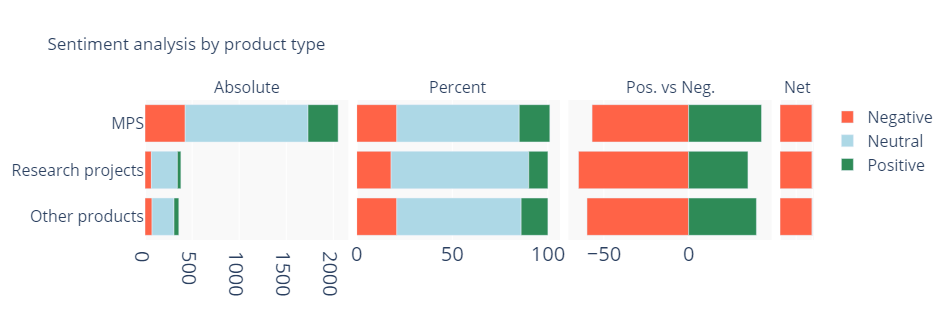
\includegraphics[width=0.95\textwidth]{Sections/images/sentiment_analysis2_2.png}}
    \caption{Sentiment analysis by product}
    \label{fig:sentiment_analysis2}
\end{figure}

MPS dominates the sentences accounting for 17 (61\%) of the 28 papers and 2051 (73\%) of the 2791 sentences analysed.

\subsubsection{A Narrative Synthesis}
Our synthesis of the papers that appear in table \ref{table:paper_key} will be short.
We will avoid rehashing the advantages and disadvantages of projectional editing, which come up again as we discussed these thoroughly in sections \ref{section:projectional_advantages} and \ref{section:projectional_disadvantages}.

Many of these papers focus on models and model-driven development, occasionally suggesting a shift towards textual modelling languages.
However, other papers point out that text does not always supply a suitable level of abstraction in modelling.
One paper suggested that developers prefer text, whereas maintainers and domain experts prefer visual projections, though this suggestion was unsourced.

When authors have used solutions other than MPS, they complain about issues such as MPS being heavyweight, with much overhead.
However, these authors then spend a great deal of time theorising about fixing issues in their architecture which, because of its architecture, MPS does not encounter.
These issues include synchronising between various views and how grammars deal with notations.

There is a fair bit of mention of a ``semi-projectional'' approach, which involves parsing at the leaf node level of the AST.
This approach is mainly from papers not using MPS, but also some which do.
The approach, it seems, is a reaction to the difficulty in simulating the text language experience in a projectional editor. 
It echoes the approach the Synthesizer Generator adopted when facing this same problem in the 80s.

The projects they describe are not in industrial use.
These authors suggest that projectional editing is probably best suited to helping novices learn a language. 

Those authors who use MPS primarily discuss products developed for use in an industrial setting or how best to teach projectional editing to a broader audience.
MPS, when used, is often seen as a critical enabler.
Two of MPS' properties that garner the most mentions are the ease of composition and multiple views.

The users of MPS agree that simulating the experience of the text editor user in the projectional environment is still very hard.
However, new plug-ins are making this somewhat more manageable.
The most prominent carrion call amongst the MPS users is for a web-based interface.

The steep learning curve is another issue.
Several papers offer solutions to this, such as example-driven development, gamification, grammar to MPS plug-ins and something called a ``language wheel''.

In general, researchers using MPS have a few gripes with usability but seem to be very positive.
One paper, which was not using MPS, said that some problems become intractable when dealing with graphical models.
Another paper, in a coincidence of word use, when describing the decision to use MPS, explained that it was because it presented a tractable level of complexity. 
